\documentclass[fr]{../../../eplsummary}

\usepackage{amsfonts}
\usepackage{pict2e}
\usepackage{framed}
\usepackage{float}

\hypertitle{Management humain}{6}{ECGE}{1321}
{Florian Thuin}
{Nathalie Delobbe}

\graphicspath{{res/}}

\section{Résume des documentaires}

\subsection{Le bonheur au travail}

On demande de plus en plus de performance et réactivité des employés
mais les structures n’ont pas évolué (coincé au stade « contrôle et
surveillance »)
La structure pyramidale n’est plus la bonne. Quels sont les modèles
alternatifs ?

\subsubsection{Vignoble « Sea Smoke » en Californie (Bob Davids)}

\begin{itemize}
    \item Bob Davids pense que plus il y a de monde dans l’entreprise moins on
s’amuse donc il ne veut que quelques employés dans son entreprise
    \item Il (Davids) ne donne pas d’ordres. C’est au directeur (donc pas lui) à
se concerter avec ses collègues pour résoudre les problèmes.
    \item Le patron (Davids) pose des questions jusqu’à ce que les employés
trouvent les réponses (il les laisser chercher eux-même)
    \item Il délègue et les autres sont aux commandes (beaucoup de confiance mais
aussi beaucoup de responsabilités)
\end{itemize}
\bigskip

Donner la responsabilité à des petits groupes c’est faisable mais
comment faire dans une grande entreprise ?

\subsubsection{Poult (fabricant de biscuits à Montauban)}

\begin{itemize}
    \item C’est une vieille entreprise donc il y a eu un passage de l’entreprise
traditionnelle à l’entreprise moderne.
    \item Entreprise traditionnelle : 
        \begin{itemize}
            \item Très hiérarchisé
            \item Culture hiérarchique directive (les exécutants robot/soldat versus les
chefs)
            \item Les employés sont très surveillés et dirigés
            \item Les employés « rebelles » sont vite envoyés dans le bureau de la
direction (style mauvais écolier)
        \end{itemize}
    \item Carlos Verkaeren (président) est un belge qui vient relancer Poult avec
une nouvelle approche innovatrice. Tous les employés se rassemblent pour
faire un brainstorming. Après des groupes de travail mis en place pour
continuer la réflexion. Il a décidé de supprimer la hiérarchie (suite à
leur perte de pouvoir beaucoup de chefs partent) et le temps n’est donc
plus passé à contrôler les employés. À la place de la surveillance, il y
a une nouvelle fonction d’accompagnement des opérateurs. Les employés
ont eu du mal à accepter les changements au début mais le succès de
Poult les a convertis assez vite.
    \item Les décisions sont prises par petits groupes. Les employés prennent les
décisions et font le planning de leur ligne de production. Pour pouvoir
faire cela il faut que l’information soit accessible à tous
(transparence).
    \item Développement d’auto-gérance, d’un sens des responsabilités, d’une
fierté de la chose accomplie. 
\end{itemize}
\bigskip

Bien sûr, tout n’est pas rose. Que fait-on du partage des bénéfices ?

\subsubsection{Entreprise Chronoflex à Nantes}

\begin{itemize}
    \item La crise de 2008 a forcé l’entreprise à mettre en place un plan social
(chose que personne ne voulait pas faire)
    \item Il veut tout changer. La pyramide est supprimée et remplacée par de
petites équipes autonomes. Ils règlent les problèmes de l’entreprise.
    \item On a demandé aux employés comment ils veulent être rémunérés ? Mise en
place d’un système de bonus à la performance individuelle mais aussi
collective en plus d’une répartition à parts égales d’une prime de
rentabilité. $\Rightarrow$ Le chiffre d’affaire a augmenté de 15\% sans rien faire
d’autre.
\end{itemize}

Chronoflex et Poult sont des entreprises dites « libérées » : Liberté et
responsabilité complète de ses actions de la grande majorité des
employés dans une entreprise donnée. \newline

Que se passe-t-il dans les services publics ?

\subsubsection{SPF mobilité en Belgique}

\begin{itemize}
    \item Base de libération : concerter les employés sur leurs aspirations
    \item Il faut changer de mode de management.
    \item Suppression du système de pointage et remplacer les horaires par
objectifs (pour motiver plus), cependant, les heures supplémentaires ne
sont pas comptées. Les employés ont donc le loisir de choisir leurs
horaires.
    \item Libérer ça veut dire aussi responsabiliser. Les personnes qui ne
travaillent pas beaucoup ne sont plus réprimandées par les supérieurs
mais par les collègues car un tire-au-flanc freine l’avance du groupe.
Critique de la part des syndicats : On tue la solidarité entre
collègues.
    \item L’espace de travail est changé : Open Space (faire tomber les murs),
    \item Dynamic office (on s’installe tous les jours où on veut. Critique : on
n’a pas sa place ?)
    \item Les avantages :
        \begin{itemize}
            \item Meilleure transparence
            \item S’asseoir avec qui on veut
            \item On peut poser des questions directement aux collèges
        \end{itemize}
    \item Les désavantages :
        \begin{itemize}
            \item Il faut trouver une place tous les matins (chaise musicale ?)
            \item L’ambiance n’est pas toujours bonne et elle affecte automatiquement tout
le monde
            \item On n’a plus de moments privés (pour prendre un rendez-vous chez le
médecin par exemple)
            \item Tout le monde voit ce qu’on fait (y compris les
                visiteurs) $\Rightarrow$ contrôle social absolu
        \end{itemize}
    \item Le directeur doit aussi rejoindre l’open space pour que tous les
changements soient cohérents. On fait face au problème de l’égo de la
hiérarchie qui est attachée aux preuves extérieures de pouvoir. Cet égo
est le pire ennemi d’une culture basée sur le bonheur au travail. 
     \item Il faut des managers sans égo qui mettent la réussite du groupe avant sa
propre réussite.
\end{itemize}

\subsubsection{“On the phenomenon of Bullshit jobs: A work rant” by
David Graeber (London School of Economics)}

\begin{itemize}
    \item Sa théorie: plus on est utile à la société moins on gagne d’argent (les
infirmières par exemple)
    \item Cercle vicieux du contrôle et de la perte d’argent
    \item Les parasites des entreprises = les non productifs (bullshit jobs)
\end{itemize}

\subsubsection{Entreprise française Favi (fonderie de fourchettes de boîtes de vitesse,
exporte dans le monde entier)}

\begin{itemize}
    \item Pas de bullshit jobs chez Favi
    \item Les employés se disent heureux et veulent se faire embaucher chez Favi.
Il n’y a même pas de syndicat.
    \item Modèle très simple : Un directeur et les employés (qui s’organisent
eux-mêmes)
    \item Règles de base de Jean-François Zobrist : 1) Confiance aux ouvriers et
aux commerciaux (bonheur et rentabilité vont de pair) 2) Amour du client 
    \item 2 principes pour que ça ne finisse pas en bain de sang :
        \begin{itemize}
            \item Améliorer l’environnement de travail (augmenter le confort, moins
d’odeurs et de fumée, augmenter la propreté et la sécurité)
            \item Créer des équipes autonomes de gens qui s’entendent bien pour gérer des
îlots de production appelé mini-usine (chacune est attachée à un client)
        \end{itemize}
    \item L’idée est de déstructurer. Chaque cellule a son propre commercial qui a
son bureau près des ouvriers au cœur de l’action (bonne chose pour la
relation commercial-ouvriers)
    \item Jean-François Zobrist dit : « la confiance rapporte plus que le
contrôle »
    \item Que se passe-t-il quand il y a un problème avec les employés ? Il y a
une première dans la mini-usine car cela impacte souvent le travail de
la cellule. 90\% des problèmes se règlent sur le terrain.
    \item Le modèle de Favi attire les gens qui aiment la responsabilité et la
liberté. Les employés doivent, puisque responsables, accepter d’être
flexibles (travailler parfois le samedi par exemple) 
    \item Zobrist s’est inspiré du concept japonais de « Kaizen » qui veut dire
amélioration continue. Il émerge au Japon après la deuxième guerre
mondiale. On respecte l’intelligence des salariés : « Celui qui fait
sait » (le mieux placé pour résoudre les problèmes est la personne qui
est sur le terrain).
    \item Urnes d’idées : Les deux meilleures sont récompensées par des prix
d’argent
\end{itemize}

\subsubsection{Harley-Davidson (U.S)}

\begin{itemize}
    \item Supprimer la bureaucratie et la remplacer par des petits groupes qui
prennent les décisions (parler ouvertement, écouter les employés). Le
plus difficile fut de faire accepter l’idée aux chefs les plus hauts
placés.
     \item Innovations $\Rightarrow$ augmentation du chiffre d’affaire
         $\Rightarrow$ les salaires et les retraites augmentent donc
         c’est bénéfique aux employés.
     \item C’est un employé qui a créé le club des propriétaires de Harley-Davidson
(20 millions de membres dans le monde actuellement)
\end{itemize}
\bigskip

Il faut faire attention aux entreprises qui prétendent faire du lean
management alors qu’il y a beaucoup de bullshit jobs.

\subsubsection{Dans les années 1950 Bill Gore, chimiste}

\begin{itemize}
    \item Il propose des idées à ses supérieurs qui refusent systématiquement.
    \item Il crée sa propre entreprise familiale.
    \item Son motto: Make money and have fun doing so.
    \item Culture Gore de confiance
    \item Les employés ont des parts dans son entreprise
    \item Il ne veut pas que nous confondions l’absence de hiérarchie avec
l’anarchie. Il y un système de leaders en place.
Le leader est un facilitateur et coordinateur qui parfois émerge
naturellement ou suite à des rassemblements où ils sont désignés par
leurs pairs.
    \item Chaque unité de travail est de maximum 250 personnes pour que les gens
puissent se connaître. Ils peuvent tous parler ouvertement car ils sont
tous collègues.
    \item L’entreprise fait du recrutement basé sur la capacité à innover et
évoluer et non sur les diplômes.
    \item Système de sponsoring par un « ancien employé » pour aider à évoluer
indépendamment du leader de chaque groupe de travail. C’est un
conseiller qui peut donner une autre perspective à l’employé qu’il
sponsorise.
    \item Le « sweet spot » de Bill Gore : Trouver le poste pour un employé où se
retrouvent les compétences/intérêts de l’employé et les besoins de
l’entreprise $\Rightarrow$ épanouissement
\end{itemize}

\subsubsection{Vineet Nayar (India), ancien président de HCL
technologies :}

\begin{itemize}
    \item « Les employés d’abord, les clients ensuite »
    \item Ancien système de dictature du chef qui fait place à un modèle de
collaboration et mentoring
    \item La pyramide étouffe la génération Y (enfants des années 80). Elle est
innovante.
    \item Pour Vineet Nayar l’argent ne fait pas le bonheur. Les gens ont besoin
de sens dans leur travail. L’argent ne motive pas à long-terme.
\end{itemize}

\subsubsection{Sillicon Valley}

\begin{itemize}
    \item Google, Yahoo, HP, Microsoft, etc.
    \item Les gens ne restent pas pour le salaire (car il est élevé dans toutes
ses boîtes) mais pour le bonheur au travail.
    \item Mais ce qui les rend heureux au travail (gym, nourriture, etc) n’est
possible que parce que ce sont des entreprises qui gagnent beaucoup
d’argent.
\end{itemize}

\subsubsection{SPF Sécurité Sociale (ministère belge)}

\begin{itemize}
    \item Frank Van Massenhove-président
    \item La génération Y ne veut pas qu’on lui dire quand et où travailler.
    \item 3 jours maximum de télétravail par semaine
    \item Réseau direct SPF : documents et chat avec les collègues disponible à la
maison
    \item Avec beaucoup de télétravail on peut faire des économies d’espace de
bureau
    \item Open Space + Dynamic Space
    \item Les employés évaluent leurs chefs et leur donnent des conseils
\end{itemize}

\subsubsection{Conclusion}

Devons-nous faire autrement ? Il faut peut-être revenir à
l’essentiel et faire plus confiance à ceux qui font.



\section{Résumé du portefeuille de texte}

\subsection{Texte 1 : Introduction au Management humain}

\subsubsection{Section 1 : Le management, l’organisation, les aspects
humains.}

Le management : action ou art de conduire une organisation, de la
diriger, de planifier son développement, de la contrôler, s’applique à
tous les domaines d’activité de l’entreprise

\begin{figure}[H]
    \centering
    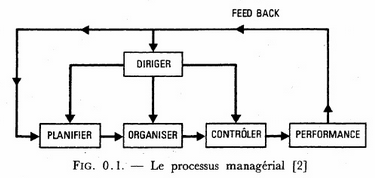
\includegraphics{processus_managerial.png}
\end{figure}

Si la tâche de planification est importante, le management ne peut être
résumé à cela. On parlera notamment, pour compléter ce que nous savons
déjà, de la main visible de Chandler. La stratégie doit conduire le
management tout en sachant que ce dernier va pouvoir l’influencer. Le
management est également destiné à transformer toute l’information, les
ressources, etc\ldots en produit ou service afin d’atteindre des
objectifs. \newline

L’organisation : D’un point de vue économique, elle rassemble les
ressources humaines et matérielles dans un même but tandis que d’un
regard social l’organisation est une réponse à l’action collective.
Les aspects humains et organisationnels du management : 

\begin{figure}[H]
    \centering
    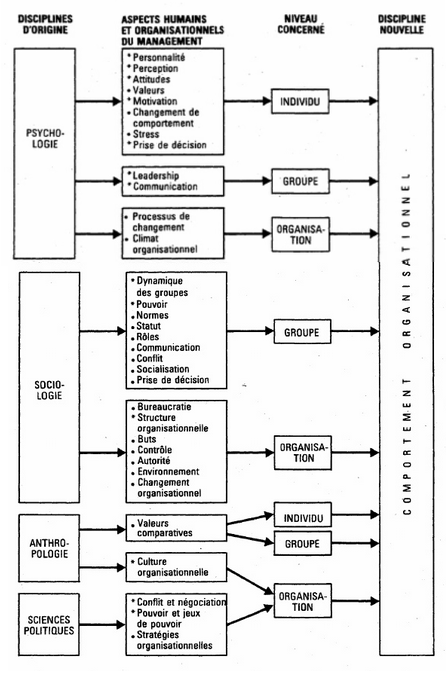
\includegraphics[width=\linewidth]{aspects_humains_et_organisationnels.png}
\end{figure}

\subsubsection{Section 2 : Les théories de l’organisation.}
A l’heure d’aujourd’hui une multitude de théories existent et cohabitent
ensemble. C’est pour quoi en définir une qui les supplanterait toutes
serait une erreur. Nous allons plutôt construire une pensée théorique
visant à positionner chaque modèle sur la carte de Scott. 

\begin{figure}[H]
    \centering
    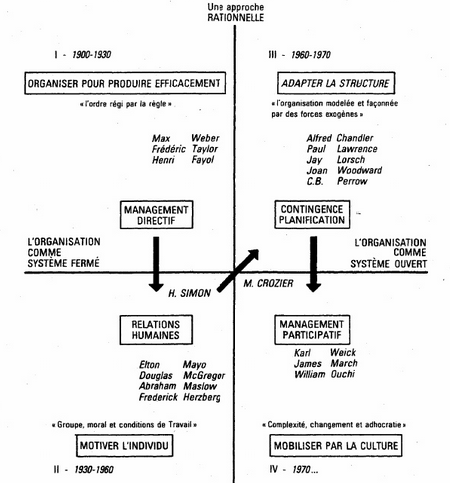
\includegraphics[width=\linewidth]{carte_de_Scott.png}
\end{figure}

\begin{description}
    \item[Zone 1] : système fermé, approche rationnelle.
Doit fonctionner seule et ce peut importe l’endroit, basé sur une
méthode scientifique.
Tout est régi par la règle et est codifié. Les hommes sont placés là où
leurs talents sont les meilleurs.
Rémunération à l’heure.
    \item[Zone 2] : système fermé, approche sociale
Si la règle est toujours bien présente, on veut redonner un visage
humain à l’entreprise. 
Lewis met en évidence les facteurs de leadership et découvre les effets
des travaux de groupes.
Il y a un travail sur la motivation des employés mais se limite à des
comparaisons psychologiques sans évocation des composantes sociologiques
ou politiques. 
    \item[Zone 3] : Système ouvert, approche rationnelle.
Les managers doivent faire avec l’environnement et adapter leurs
solutions.
Pour s’adapter au mieux à l’environnement on cherche à trouver la
structure qui mélange au mieux centralisation et décentralisation
    \item[Zone 4] : système fermé, approche sociale
L’acteur social remplace l’acteur rationnel.
La culture de l’entreprise commence à être reconnue et devient
importante. Une action chaotique est préférable à l’inaction.
On favorise la prise d’initiatives.
\end{description}


\subsubsection{Section 3 : Eléments de méthode.}
Si la science managériale peut se développer c’est uniquement parce que
les managers et les scientifiques collaborent. Nous allons à présent
décrire ce que nous entendons par théorie et présenterons ensuite les
méthodes de recherches les plus utilisées en tentant de dresser leurs
avantages et faiblesses. \newline

Théorie : ensemble de règles qui permet d’expliquer un grand nombre de
faits.  Selon Miner, une bonne théorie est « capable d’aider la science
en aidant à la compréhension de la question posée, possède des limites
d’application, incite à d’autres recherches, produit des résultats que
l’on peut généraliser, est sujette à des remises en causes, est énoncée
de façon simple ». \newline

Avantages de la méthode scientifique : 

\bigskip
\begin{itemize}
    \item Les connaissances sont publiques et donc peuvent être regroupées et
stockées. 
\item Les procédures sont construites de façon à pouvoir être répétée et sont
donc objectives. 
\item L’élaboration de la théorie se fait sur base de ce qui est connu et sur
de nombreuses observations. 
\item Les échantillons sont représentatifs.
\item Les objectifs sont clairs et précis et se veulent explicatif de lien
causal. 
\end{itemize}
\bigskip

La méthode scientifique : 

\begin{figure}[H]
    \centering
    \begin{minipage}{0.4\linewidth}
        \centering
        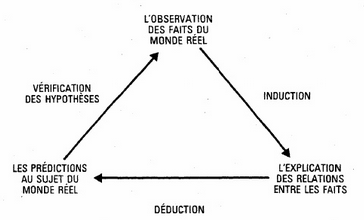
\includegraphics[width=\linewidth]{methode_scientifique.png}
    \end{minipage}
    \begin{minipage}{0.4\linewidth}
        \centering
        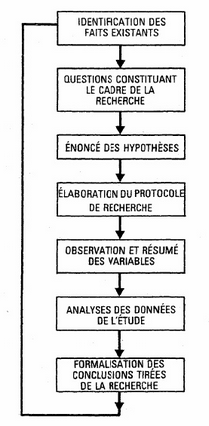
\includegraphics[width=0.6\linewidth]{methode_scientifique_2.png}
    \end{minipage}
\end{figure}

Les principales méthodes de recherches : 

\begin{itemize}
    \item L’observation naturelle : On observe des indiivuds ou des groupes
longtemps avant de tirer des conclusions. Ce type d’observation peut
être qualifiée de naturelle par experts (des experts rédige la théorie
sur base de leur observations et vécu) ou par la dénomination étude de
cas (on analyse un cas afin de pouvoir traiter un problème général).
    \item Le sondage : on utilise un questionnaire standardisé afin de mesurer
certains variables utiles à la prise de décision.
    \item L’étude de terrain : elle permet l’étude de corrélation entre plusieurs
variables. Elle se base sur des observations et une méthodologie
rigoureuse. 

\begin{figure}[H]
    \centering
    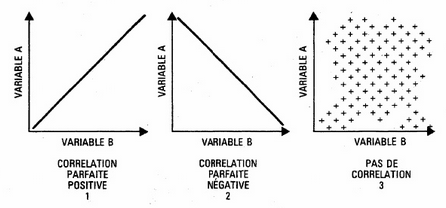
\includegraphics[width=0.5\linewidth]{correlation_etude_de_terrain.png}
\end{figure}

    \item L’expérience de terrain : se rapproche fortement de l’étude de terrain à
la différence qu’ici on va modifier de façon intentionnelle
l’environnement ou une variable. 
    \item L’expérience en laboratoire : on isole les variables que l’on veut
mesurer ou voir évoluer
\end{itemize}

\begin{figure}[H]
    \centering
    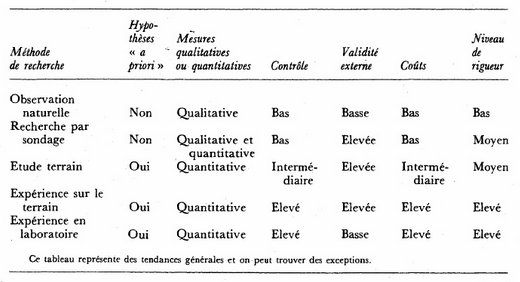
\includegraphics[width=0.7\linewidth]{experience_laboratoire.png}
\end{figure}

Avantages et faiblesses des méthodes : 

\begin{figure}[H]
    \centering
    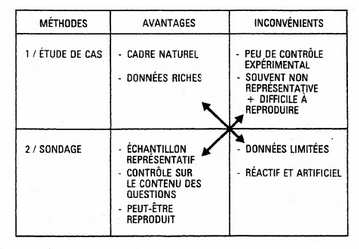
\includegraphics[width=0.6\linewidth]{avantages_faiblesses_methode.png}
    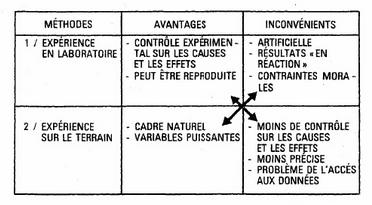
\includegraphics[width=0.6\linewidth]{avantages_faiblesses_methode_2.png}
\end{figure}



\subsection{Texte 2 : Human resource roles.}

\subsubsection{Section 1 : Perspective historique des HR.}
Les ressources humaines sont en train de passer d’une fonction simple et
isolée dans l’entreprise à quelque chose de beaucoup plus important avec
une augmentation de l’impact dans la prise de décision et dans la
stratégie. Selon Miles et Snow (1984)le rôle des HR était surtout lié au
recrutement et à la gestion du personnel. Par la suite on a ajouté la
fonction de « coach », les HR doivent également s’occuper de la
formation précise des employés. Selon Friedman la partie technique de la
chose était l’attribution des salaires, le design du packaging de
rémunération, etc.. Par après, dans les années 70, est apparue la
fonction de DRH avec 3 axes d’action : éducation, training et
développement.

\subsubsection{Section 2 : Priorités et focus de la fonction RH.}
Jusqu’à aujourd’hui, l’accent de la fonction des RH était mis sur
l’activité opérationnelle. Il fallait que les employés soient
opérationnels, qu’ils travaillent en étant heureux, etc… Aujourd’hui on
remarque que de plus en plus, la fonction des RH s’apparente à de la
stratégie.

\subsubsection{Section 3 : Nouveaux rôles et compétences}
Walker a noté une continuité entre 4 types de rôles : support ;
service ; consulting et leadership. En 1990, Schuler a noté que le rôle
des RH est devenu encore plus important et fait intégralement partie de
la stratégie. Il définit 6 rôles : buisiness person ; shaper of change ;
consultant/partner to line; formuler la stratégie et l’implémenter;
talent manager, cost controller et asset manager. Wiley pour sa part
classifie les HR en trois structures : le processus stratégique ;
l’aspect légal et aspects opérationnels.

\begin{figure}[H]
    \centering
    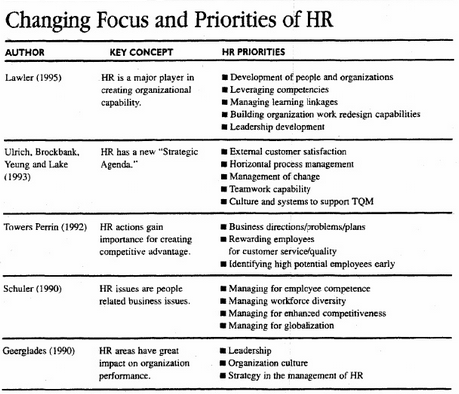
\includegraphics[width=\linewidth]{focus_priorities_HR.png}
\end{figure}

\subsubsection{Section 4 : HR role framework (Ulrich, 1993).}

\begin{description}
    \item[Le rôle de strategic partner] : On allie le travail des HR avec le
travail stratégique. 
    \item[Le rôle d’expert administratif] : Ce rôle représente les fonctions
traditionnelles des HR. Il concerne également la construction des
structures RH. 
    \item[Le rôle d’agent de change] : C’est un rôle très important car il va
permettre à l’entreprise de trouver les moyens de rester compétitive. 
    \item[Le rôle d’employee champion] : Cette fonction s’occupe des problèmes au
jour le jour des employés et fait en sorte que tout se passe pour le
mieux. Elle gère le moral et la motivation des travailleurs. 
\end{description}
\bigskip

Avec ces nouveaux rôles et ces nouvelles fonctions, il faut de nouvelles
compétences. On en a identifié trois jeux : savoirs lié à l’activité de
l’entreprise ; les ressources humaines et le management des processus de
changement. \newline
Le reste du texte est dédié à la description du protocole qui a permis
de dresser la carte des attentes pour chaque rôle. 

\begin{figure}[H]
    \centering
    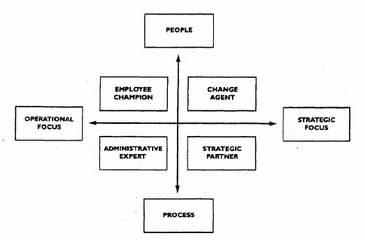
\includegraphics[width=\linewidth]{ulrich_role_framework.png}
\end{figure}

\subsection{Texte 3 : La culture organisationnelle.}

\subsubsection{Section 1 : Le concept de culture
organisationnelle.}

C’est au début des années 80 qu’apparait véritablement le concept de
culture organisationnelle. Plusieurs facteurs et courants sont à
l’origine du développement du concept. Tout d’abord, Mayo dans les
années 30, a démontré que les agents répondaient plus à l’interprétation
qu’ils avaient des choses plutôt qu’à des objectifs et ordres clairs et
concis. Weik a poursuivi avec ses travaux qui ont su prouver que le
modèle bureaucratique ‘n’était pas la base, ne constituait pas le
mécanisme de cohérence de toute entreprise. \newline 

Une définition : Programmation collective de l’esprit qui définit les
façons de penser, de ressentir et d’agir et qui distingue les membres
d’un groupe ou d’une catégorie de personnes des autres groupes ou
catégories de personnes.\newline

L’entreprise a une culture : Comme la structure, chaque entreprise
possède sa culture propre et celle-ci est une variable au même titre que
les autres. Alors les scientifiques font en sorte de définir les
composantes de cette variables afin de voir les liens existant avec le
reste de l’organisation. La culture est un attribut qui vient se
superposer à ce qu’est l’entreprise. On peut voir la chose comme une
variable dépendante (selon le pays, etc…) ou indépendante (attribut
produit par l’entreprise afin d’assurer sa régulation et sa cohésion
sociale). \newline

L’entreprise est une culture : Lorsque la culture est considérée comme
une grille de lecture permettant de donner sens à l’ensemble des
phénomènes organisationnels. \newline

Les différentes strates de la culture organisationnelle : Toute culture
orga repose sur des strates qui sont profondes ou changeantes. Selon le
modèle de l’oignon, il y a 3 ou 4 strates. La première, les points
fondamentaux, se base sur les relations humaines et sur les liens
existant entre toute chose. Sur cette base s’articule un ensemble de
valeurs qui vont pousser soit à la compétitivité ou à la solidarité. La
troisième strate représente les normes de pensée et d’action. Ce sont
les routines et procédures, façon de réagir devant tel ou tel type
d’évènement. Enfin arrive la dernière strate qui distingue l’entreprise,
les artefacts. Ce sont les manifestions matérielles des pensées et
valeurs (logos, noms d’objets, règlements, etc\ldots).

\begin{figure}[H]
    \centering
    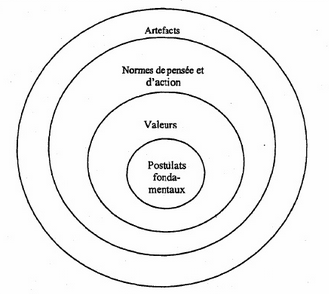
\includegraphics[width=0.4\linewidth]{modele_de_schein.png}
\end{figure}

\subsubsection{Section 2 : Le modèle des valeurs concurrentes de Quinn
(1988).}

Le modèle, bien que crée à la base pour décrire les valeurs
sous-jacentes aux critères d’efficacité organisationnelle, caractérise
les cultures organisationnelles selon deux dimensions : l’orientation
des entreprises (interne ou externe) et le niveau de flexibilité. 

\begin{figure}[H]
    \centering
    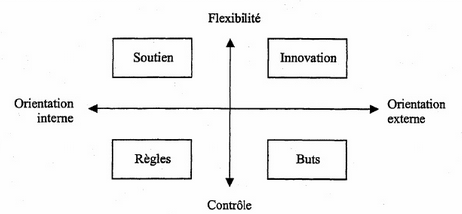
\includegraphics[width=0.8\linewidth]{modele_de_quinn.png}
\end{figure}

La culture « Soutien » : Soucieuses du bien-être de leur membres, ces
sociétés prônent la coopération et la participation. La communication y
est très importante et il y a de nombreux rdv informel. Il faut que les
membres attachent une importance à l’entreprise. 
La culture « Innovation » : La formalisation est peu présente ca race
sont des entreprises qui veulent favoriser la créativité, etc… Ces
entreprises renouvellent souvent leurs produits et processus/structures. 
La culture « Règles » : Structure hiérarchique et division du travail
très fortement développée. Respect de l’autorité et communication
hiérarchique. 
La culture « Buts » : Tournées vers le succès, ces entreprises
favorisent la planification, le développement par objectifs, le système
de récompenses, etc\ldots

\subsubsection{Section 3 : Construction de la culture
organisationnelle.}

L’environnement sociétal : la plupart des cultures et croyances qui vont
influencer et construire la culture de l’organisation au niveau des
individus viennent du développement personnel de ces dits individus.
Leurs croyances personnelles sont apparues au fur et à mesure des
années. \newline

Les contingences liées au secteur d’activité : la culture de
l’entreprise est également façonnée par le milieu dans lequel elle se
développe comme la scène sur laquelle elle se développe ou l’industrie
dans laquelle elle est active. \newline

L’histoire et les fondateurs : l’histoire de l’entreprise joue également
un rôle dans la construction de la culture. \newline

La culture comme construction sociale : Au travers des échanges
quotidiens, la culture va se créer et donner un cadre de référence
servant à faire disparaitre les incertitudes et porteur d’identité
situationnelles. Aussi certains ont plus de pouvoir vis à vis de
l’influence sur la culture que d’autres. La culture est donc également
un instrument de légitimation au service d’intérêts particuliers. 

Perpétuation culturelle et pratiques du management : Sathe (1985).
Le modèle postule sur le fait que les nouveaux individus recrutés sont
déjà en partie en accord avec les valeurs de l’entreprise et qu’’ils
seront soumis à une période test après laquelle ils partiront
volontairement ou non en fonction de leur adhérence aux valeurs. Par la
suite, la culture va réguler les comportements et avec un minimum de
vérification et de contrôle des comportements qui n’adhèreraient pas
encore entièrement, on va pouvoir imposer de façon subtile la culture de
l’entreprise (via le jargon, les procédures, etc\ldots)

\begin{figure}[H]
    \centering
    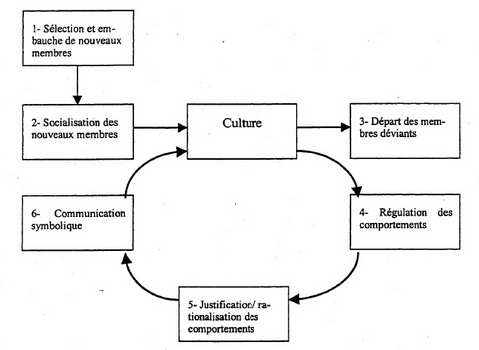
\includegraphics[width=\linewidth]{modele_de_sathe.png}
\end{figure}

Schneider (1987). De par des recherches, il a été découvert qu’il y a
également des sous-cultures d’entreprises. Celles-ci peuvent par exemple
être liées au corps de métiers et être en conflit avec celles
généralement prônées par les organisations. \newline

La culture de l’entreprise peut également se heurter à la culture
nationale qui est constituée de quatre éléments distincts : la distance
au pouvoir (si elle est forte alors la hiérarchie est très respectée) ;
l’évitement de l’incertitude ; la masculinité/féminité (si masculin
alors différentiation des sexes) ; l’individualisme/collectivisme.

\subsubsection{Section 4 : Les répercussions de la culture
organisationnelle.}

Après plusieurs études empiriques, il est impossible de dire si un type
de culture impacte plus les résultats qu’un autre. On peut par contre
affirmer qu’il existe un lien entre le type de culture et certains types
de performances. On peut également dire qu’à court terme, une
homogénéité de culture est favorable à la performance. \newline

Un fait remarquable est l’impact de la culture sur l’individu. En effet,
si les valeurs de l’entreprise sont proches, en adéquation avec celle du
travailleur celui-ci va voir sa motivation être augmentée et sa réussite
personnelle améliorée. Dans une perspective situationniste, il apparait
que les employés sont plus satisfaits dans les cultures fortes et
centrées sur les personnes. 


\subsection{Texte 4 : Le leadership} 

\subsubsection{Section 1 Les approches traditionnelles du leadership.}
Le leadership en tant que rôle : Selon Fayol il existe cinq rôles que
l’on peut attribuer à un manager. Par la suite, on les a noté sous forme
de quatre référentiels : planification ; organisation ; commandement et
contrôle.  Mitzberg qui était d’abord contre, a finalement défini 10
rôle au manager et les a classer en 3 catégories : représentation ;
information ; décision.
Le leadership, un style : On fait la différence entre les tâches et le
côté humain. Mc Gregor a défini son modèle X ( modèle considérant les
personnes comme paresseuses et qui fonctionne sous la contrainte) et Y
(les gens veulent se réaliser dans leur travail et on peut donc
travailler avec eux sans les contraindre). Par la suite, on a défini le
modèle des 4S.

\begin{figure}[H]
    \centering
    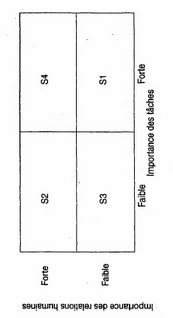
\includegraphics[angle=270, width=0.6\linewidth]{modele_4S.png}
\end{figure}

S1 : Contrôle est absolu et on travaille avec la contrainte et les
ordres stricts. Le manager travaille derrières les travailleurs et les
surveille constamment. 
S2 : Style « convivial » il va favoriser le côté humain tout en gardant
le contrôle. Dans ce style on trouve plus d’autonomie. 
S3 : Style « laisser faire ». Le manager est là sans être là et joue le
rôle de transmetteur. 
S4 : Style idéal qui est considéré comme guide et consultant. 
Le leadership VS management : Selon Kotter, le leadership équivaut au
changement et possède trois fonctions : définir une direction, aligner
les salariés, motivation. Le management est lié à la complexité et
possède également trois fonctions : planification et budgétisation ;
organisation et affectation des personnes et contrôle+ résolution des
problèmes. 
Le leadership selon l’approche des compétences : Le management est l’art
de savoir ce qui doit être fait et comment le faire. Le leadership
consiste à savoir ce qu’il faut faire et à prendre la décision de si
quelque chose doit être fait ou non. Ces compétences sont liées à la
vision positive du futur, avoir une bonne image de soi et savoir comment
cela doit être fait. Le leader apprend aux autres. 

\subsubsection{Section 2 : Qu’est-ce que le pouvoir ?}

Définition : Le fait qu’A puisse obtenir de B une action qu’il n’aurait
pas faite tout seul. \newline

Les différents types de pouvoir : 

\begin{description}
    \item[Pouvoir statutaire] : le pouvoir est attaché et lié à une fonction. La
personne qui le détient peut user des récompenses, sanctions, moyens
financiers et matériels ainsi que de l’information officielle pour
l’exercer. 
    \item[Pouvoir organisationnel] : C’est le pouvoir lié à l’incertitude. Si l’on
devient expert dans une fonction qui est incertaine ou si l’on détient
des informations qui ne peuvent s’acquérir que par la pratique et qu’on
est les seuls à les détenir, on obtient ce genre de pouvoir et l’on peut
commencer à négocier. 
    \item[Le pouvoir personnel] : Ce pouvoir vient de l’admiration des autres et de
leur dévotion envers-vous. On attribue ce pouvoir aux personnalités
charismatiques. Ce pouvoir est lié à la capacité de provoquer chez les
autres ce que l’on appelle un « transfert ». Ce transfert peut être de
trois types : paternel (on donne une image protectrice et bienveillante
du manager) ; maternel (image d’empathie)  ou fraternel (image
critique). A noter que le transfert va dans les deux sens et qu’il peut
avoir un versant négatif comme la création d’un complexe d’\oe dipe. 
\end{description}

\subsection{Texte 5 : La dynamique de groupe} 

\subsubsection{Section 1 Qu’est-ce qu’un groupe ?}
Un groupe est l’association de d’au moins deux individus afin de
réaliser un objectif commun. Il y a des groupes formels et informels.
Ces derniers n’ont pas de structure clairement établie par
l’organisation.  \newline

On peut également définir d’autres types de groupes : 

\begin{itemize}
    \item Hiérarchique
    \item De travail (les individus travaillent tous sur la même tâche)
    \item D’intérêt (on travaille pour un objectif profitable à tous ceux du
groupe)
    \item D’affinité (les gens partagent des point communs)
\end{itemize}

Pourquoi construire un groupe : Besoin de sécurité ; statut ; estime de
soi ; appartenance ; pouvoir ; réalisation d’objectif.

\subsubsection{Section 2 : Les étapes de la dynamique de groupe.}

Le modèle à cinq étapes : 

\begin{enumerate}
    \item Formation (incertitude concernant la structure, les leaders, les
buts).
    \item Agitation (conflit interpersonnel jusqu’à la définition d’une
hiérarchie claire)
    \item Cohésion (Normalisation et stabilisation du mode de fonctionnement)
    \item Performance (les membres se connaissent et le groupe devient
efficient)
    \item Dissolution ( le groupe se disperse, les réactions varient d’une
personne à l’autre)
\end{enumerate}

Défaut de ce modèle : il ne prend pas en compte l’organisation ou
l’environnement dans lequel s’inscrit ce groupe. 

\begin{figure}[H]
    \centering
    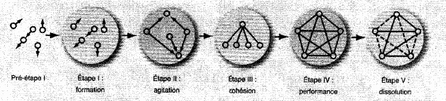
\includegraphics[width=0.7\linewidth]{etapes_vie_groupe.png}
\end{figure}

Un modèle alternatif pour les groupes temporaires : modèle d’équilibre
ponctuel.

\begin{figure}[H]
    \centering
    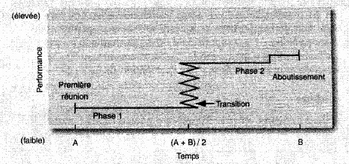
\includegraphics[width=0.7\linewidth]{modele_equilibre_ponctuel.png}
\end{figure}

\subsubsection{Section 3 :  Caractéristiques du groupe.}

\begin{description}
    \item[Les rôles] : comportement prévisible d’une personne qui occupe une
position donnée dans un contexte social donné.
    \item[L’identité de rôle] : attitudes et comportement attendus d’un rôle.
Perception de rôle : idée qu’un individu se fait de la façon dont il est
censé se comporter dans une situation donnée. 
    \item[Les attentes de rôle] : idée que les autres se font quant au comportement
qu’une personne doit adopter dans une situation donnée. 
    \item[Le contrat psychologique] : accord tacite qui définit ce qu’un employeur
attend de ses employés et vice versa. 
    \item[Conflit de rôle] : situation dans laquelle les attentes correspondant à
des rôles différents divergent. 
\item[Les normes] : attitude à avoir lorsque l’on est dans un groupe. On peut
diviser les normes en 4 catégories : performance (quotas, façon de
faire, etc\ldots) ; apparence (tenue vestimentaire, loyauté, etc\ldots) ;
interactions sociales  et attribution des ressources (salaires,
etc\ldots)
\item[La conformité] : action d’ajuster son comportement de façon à s’aligner
sur les normes du groupe.
\item[Groupe de référence] : groupes les plus importants auxquels les individus
appartiennent ou souhaitent appartenir et pour lesquels ils acceptent de
se conformer aux normes. 
\item[Comportements professionnels déviants] : actes antisociaux de certains
membres de l’organisation qui violent intentionnées les normes établies
et nuisent à l’organisation ou a ses membres voire au deux. 
\item[Statut] : place ou rang occupé au sein d’un groupe et conférant un
certain prestige ; ensemble des attributs liés à une position dans un
système culturel ou un groupe donné. 
Avec le statut, vient la confiance. On remarque que les gens dont le
statut est plus élevé ont plus facile à communiquer, sont plus
confiants, etc\ldots Les statuts et l’importance qu’on leur donne varient
d’une culture à l’autre et donc pour un dirigeant, il est important de
bien connaitre ce genre de chose s’il ne veut offusquer les membres de
son équipe. 
\item[La taille d’un groupe] : La taille joue un rôle non négligeable sur
l’efficience d’un groupe. On remarque par exemple que les petits groupes
vont réaliser leur tâche plus rapidement, mais que les grands groupes
s’en sortent mieux pour trouver des solutions à un problème. 
\item[La paresse sociale] : tendance à fournir moins d’efforts et à diminuer
son rendement au sein d’un groupe en situation de travail collectif. 
\item[Cohésion] : force qui unit les membres d’un groupe et les incite à y
demeurer ; résultat du désir des membres d’un groupe d’appartenir à ce
groupe et de leur motivation à y maintenir une participation active. 
\end{description}

\begin{figure}[H]
    \centering
    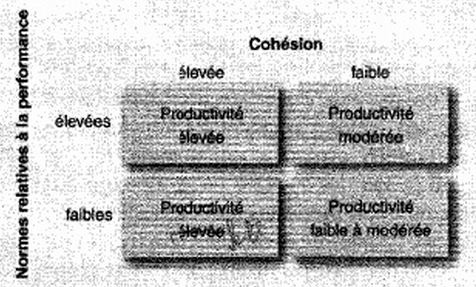
\includegraphics[width=0.6\linewidth]{caracteristiques_groupe.png}
\end{figure}

\subsubsection{Section 4 : La prise de décision collective}

\paragraph{Collectif contre individuel}

\textit{Les atouts de la décision collective} : plus d’informations et d’idées
pour prendre la décision ; la décision est plus pertinente et plus vite
accepté. \newline
\textit{Les faiblesses} : ambiguïté quant à la responsabilité ; collaboration
forcée ; il faut plus de temps. Il y a toujours des leaders et s’ils
sont médiocres alors c’est toute l’efficacité du groupe qui en pâti.
\newline

Il ressort également que les groupes sont plus efficaces sur la
précision des choses, la créativité et l’acceptation des décisions. Ils
sont néanmoins plus lents excepté lorsqu’il faut récolter un nombre
important de données ou contacter un  nombre important de personnes.
\newline 

\paragraph{La pensée de groupe} : tendance des membres à dissimuler une opinion
divergente ou minoritaire voire à perdre tout sens critique sous la
pression des normes de conformité. \newline

\paragraph{Déplacement de groupe} : caractérise la valorisation de prise de risque
entre une décision collective et une décision individuelle ; soit chacun
renforce sa position initiale soit les membres osent une prise de
risque. \newline

Les différentes techniques de travail en groupe :

\begin{enumerate}
    \item Le Brainstorming
    \item La technique du groupe nominal : mélange entre discussion de groupe
et actes anonyme. On attribue une note de façon anonyme aux idées et
c’est celle qui a le plus de points qui gagne. 
    \item TGAO : comme la technique nominale mais avec des ordinateurs. 
\end{enumerate}

\begin{figure}[H]
    \centering
    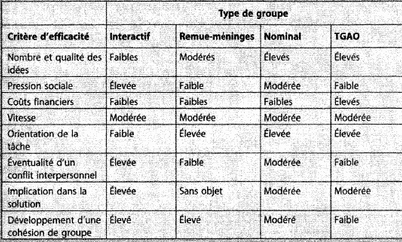
\includegraphics[width=\linewidth]{techniques_travail_groupe.png}
\end{figure}

\subsection{Texte 6 : La motivation au travail} 

\subsubsection{Section 1 Définition de la motivation au travail.}

La motivation est l’énergie investie volontairement et de façon durable
par un individu et orientée vers un but dont l’atteinte lui procure
satisfaction. On retiendra donc que la motivation est constituée d’au
moins 4 caractéristiques juste par cette définition : volontariste ;
durable ; orientée ; satisfaction. \newline

La motivation et la performance ne vont pas forcément de pair

\bigskip
\begin{tabular}{|p{0.45\linewidth}|p{0.45\linewidth}|}
\hline
    Motivé et performant : cas le plus souhaitable &
Pas motivé, mais performant : l’employé ne retire aucun intérêt à ce
qu’il fait et est performant soit parce que trop qualifié soit parce que
tout le temps controlé. \\ \hline
Motivé et non performant : l’employé veut faire ses preuves, mais n’en a
pas les capacités (mauvaise place ; mauvaise pression, environnement
laxiste, etc\ldots) & 
Ni motivé, ni performant : situation peu souhaitable. A noter que cette
situation peut être passagère chez certaine personne à cause de
problèmes personnels. \\
\hline
\end{tabular}
\bigskip

\subsubsection{Section 2 : L’historique des recherches sur la
motivation.}

De 1900 à 1925 : la motivation économique. Nous sommes dans une période
où les gens sont peu instruits et où l’on pense que faire correspondre
un intérêt monétaire avec un objectif à atteindre est la bonne solution.
Taylor et l’organisation scientifique du travail. \newline

De 1925-1950 : la motivation par la satisfaction des besoins. Durant
cette période on fait énormément de recherches pour savoir s’il n’y a
vraiment que l’apport financier qui motive les gens à travailler. On se
rends évidemment compte que non, il y a plus. Il y a la variété des
tâches, l’autonomie, etc\ldots De là quelques grandes théories et expériences
émergent. \newline
De 1950 à 1975 : l’influence de l’environnement sur la motivation. Les
recherches changent de cap. Il n’est plus question de se concentrer
uniquement sur l’individu, mais bien sur l’environnement dans lequel il
évolue. La motivation pourrait-elle venir des tâches challengeant ou
alors de la bonne relation au sein d’une équipe, etc\ldots \newline

De 1975 à 2000 :  variation sur un même thème. On approfondi ce qui a
été découvert au siècle passé. \newline 

\subsubsection{Section 3 : Les théories sur la motivation.}
La motivation par la satisfaction des besoins de croissance : 
On revient sur la théorie des beosins de Maslow qui dit qu’une fois q’un
besoin est satisfait il faut mettre en place les moyens de satisfaire le
besoin qui va suivre. Après, on revient sur la théorie X et Y qu’on a
déjà évoqué dans une lecture précédente. \newline

La théorie ERG : Existence, relation et croissance. Cette théorie est
assez proche de celle de Maslow mais vient la compléter avec l’idée de
frustration- régression qui dit que si l’on est incapable de satisfaire
un besoin alors on va se sentir frustré et on va vouloir redescendre
dans notre pyramide de besoin pour essayer de satisfaire des besoins
d’un autre type. 

\begin{figure}[H]
    \centering
    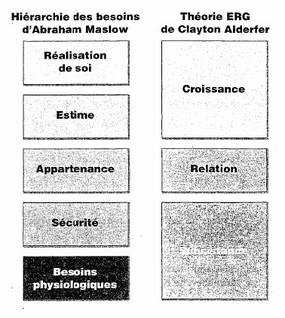
\includegraphics[width=0.4\linewidth]{maslow_aldefer.png}
\end{figure}

La théorie des deux facteurs de Herzberg : Théorie postulant l’existence
de deux catégories de facteurs dont seuls ceux qui sont de nature
intrinsèquement satisfaisante (facteurs motivateurs) ont la capacité de
mobiliser les employés. Les autres facteurs, dits d’hygiène, ont pour
fonction de prévenir le mécontentement sans pour autant conduire à
performer.  \newline

Il y a tout de même des limites à cette théorie. La façon dont les
questions ont été posées induise une réponse plutôt qu’une autre. Les
employés s’attribuent le crédit en cas de réussite et blâment les autres
en cas d’échec. Il n’y a pas de mesure générale de la satisfaction. Ce
n’est pas vraiment une théorie sur la motivation mais plutôt une théorie
explicative des facteurs de satisfactions. 

\begin{figure}[H]
    \centering
    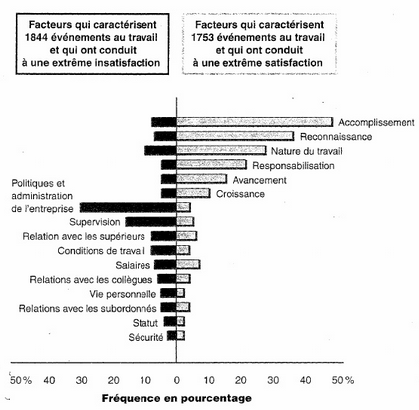
\includegraphics[width=0.8\linewidth]{facteur_satisfaction.png}
\end{figure}

\paragraph{Les quatre besoins humains}

\begin{itemize}
    \item Le besoin d’acquérir et de conserver. 
    \item Le besoin d’entrer en relation.
    \item Le besoin d’apprendre.
    \item Le besoin de défendre.
\end{itemize}

\paragraph{La théorie des attentes}

Jusqu’ici on a dit que la motivation venait d’un besoin de satisfaction.
Vroom a cependant affirmer que la motivation pouvait également être
rationnelle et qu’il était possible d’orienter les gens sur la seule
base de leur attente. La théorie des attentes est une théorie de
motivation selon laquelle les individus croient que leurs efforts les
conduiront à atteindre un certain niveau de performance qui est lui-même
lié à un résultat et à une source de récompensent qu’ils valorisent. Il
y a également un autre élément important dans cette théorie : les
valences. On accorde en effet une certaine valence aux choses et cette
valence peut-être positive ou négative. Si par exemple on aime notre vie
et qu’on nous propose une promotion qui va nous demander plus d’heures
de travail on va pouvoir considérer une valence négative pour cette
proposition. 

\begin{figure}[H]
    \centering
    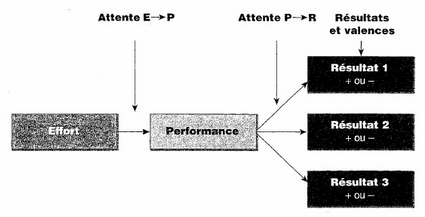
\includegraphics[width=0.6\linewidth]{theorie_attentes.png}
\end{figure}

D’autres théories ont été émises comme celle prônant la définition
d’objectifs afin de motiver les employés. Un élément important saute
alors aux yeux : la rétroaction (information qu’une personne reçoit sur
ses performances). La rétroaction possède des caractéristiques claires
et importantes vis-à-vis de sa bonne compréhension. 

\begin{figure}[H]
    \centering
    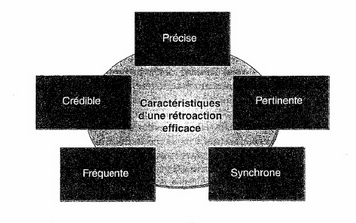
\includegraphics[width=0.5\linewidth]{theorie_retroaction.png}
\end{figure}

\end{document}
